% Secao de resultados preliminares. As figuras estao em docs/figuras/ e saem de
% scripts/figuras_resultados.py; os numeros, das saidas da semana coletada.

\section{Resultados preliminares}
\label{sec:resultados}

A coleta foi executada entre 02/09/2026, 19h22, e 09/09/2026, 19h22, sobre as
linhas 3459, 4310, 5300, 6000, 6091, 6450, 6500, 6913, 8400 e 8594, nos dois
sentidos, escolhidas por terem previsão de chegada publicada pela API em ao
menos 40\% das paradas do itinerário. As posições de toda a frota foram
consultadas a cada 30~s e as previsões das linhas monitoradas, a cada 60~s. Como
a API não informa o instante em que o veículo chega à parada, esse instante foi
reconstruído projetando posições e paradas sobre o traçado do GTFS
\cite{gtfs:2026} e interpolando o momento em que o veículo cruza cada parada
\cite{cathey:2003}. Dos 90,0 milhões de
posições e 15,8 milhões de previsões coletadas, resultaram 451.409 chegadas,
421.325 trechos com tempo de referência, distribuídos em 17.450 viagens, e
12.982.114 pares entre previsão e chegada\footnote{Painel interativo com os
resultados: \url{https://onibus.tagg.chat}. Os conjuntos de dados estão
disponíveis no repositório do projeto.}.

\subsection{Caracterização do atraso}

Cada observação corresponde a um veículo percorrendo um trecho entre duas paradas
consecutivas, cujo tempo típico é de 81~s. Com a referência dada pela mediana do
mesmo trecho, sentido e faixa horária, a mediana do atraso é nula por
construção, e a informação relevante está na cauda da distribuição: 24,4\% dos
trechos ficaram ao menos 20\% acima da referência, e o percentil 90 do atraso
(p90) é de 40,5~s. Por trecho, o desvio é pequeno, mas se acumula ao longo da
viagem: das 15.755 viagens com ao menos dez trechos, 32,4\% acumularam 5~min ou
mais acima do tempo típico, e 17,0\%, 10~min ou mais.

\subsection{Padrão temporal}

A Figura~\ref{fig:perfil} mostra que o atraso é sistematicamente maior em dias
úteis: a proporção de trechos atrasados cai de 28,3\% nos dias úteis (p90 de
47,9~s) para 19,4\% aos sábados (29,3~s) e 12,1\% aos domingos e no feriado de
07/09 (18,5~s). Nos dias úteis, os horários de pico (6h--8h e 16h--19h)
concentram a cauda do atraso, com 30,6\% de trechos atrasados e p90 de 58,8~s,
contra 26,9\% e 41,9~s fora deles, e a velocidade mediana atinge o mínimo de
17,6~km/h às 18h, contra cerca de 31~km/h na madrugada. Na escala da viagem, o
efeito é mais nítido: 42,9\% das viagens do pico da tarde acumularam 5~min ou
mais de atraso, contra 15,9\% das realizadas de madrugada.

\begin{figure}[ht]
\centering
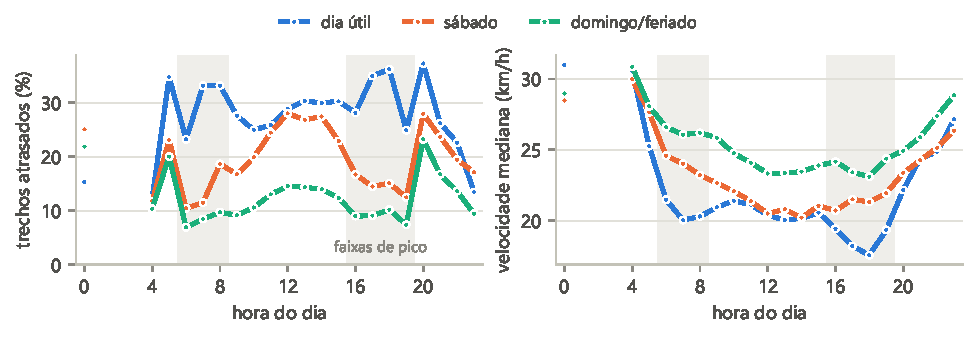
\includegraphics[width=\textwidth]{figuras/perfil-dia.pdf}
\caption{Trechos atrasados (esquerda) e velocidade mediana (direita) por hora e
tipo de dia. Faixas cinzas: picos; lacuna entre 1h e 4h: pausa da coleta.}
\label{fig:perfil}
\end{figure}

O pico de 37,3\% às 20h decorre da referência por faixa horária: a noturna é
dominada pelas horas mais vazias, e o trânsito remanescente do pico fica acima.

\subsection{Distribuição espacial e paradas críticas}

A Figura~\ref{fig:mapa} mostra, por parada, o p90 do atraso relativo ao tempo
típico do trecho e a velocidade mediana. A normalização é necessária porque o
p90 em segundos acompanha o tamanho do trecho (correlação de 0,96 com o tempo
típico, por linha): as linhas 5300, 6500 e 6450, de paradas mais espaçadas, têm
os maiores valores absolutos (cerca de 58~s), mas, em proporção do tempo típico,
a 5300 é a mais regular (39\%) e a 6500 a menos regular (48\%)
(Tabela~\ref{tab:linhas}). As mais lentas são a 8400 e a 8594, entre o centro e
a zona norte-oeste, abaixo de 19~km/h. Entre os fluxos de origem e destino com
ao menos mil trechos, a proporção de atrasados varia de 21,4\% a 26,1\%, e o p90
relativo, de 36,5\% (Varginha $\rightarrow$ Itaim Bibi) a 49,8\% (Bandeira
$\rightarrow$ Santo Amaro). Entre as paradas com ao menos 300 trechos, o p90
passa de 1,6 vez o tempo típico no SESC Pompeia e na Av.~Alcântara Machado, na
Radial Leste; na R.~Itajuibe chega a 4,2 vezes, o que sugere espera programada
e ainda será verificado.

\begin{figure}[ht]
\centering
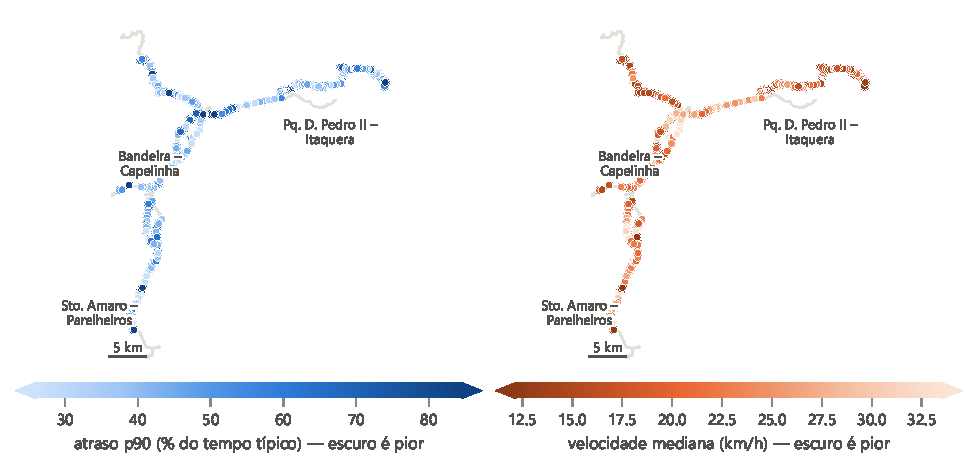
\includegraphics[width=0.8\textwidth]{figuras/mapa-paradas.pdf}
\caption{Atraso p90 em proporção do tempo típico do trecho (esquerda) e
velocidade mediana (direita) por parada com ao menos 100 trechos. Cores escuras
indicam pior desempenho.}
\label{fig:mapa}
\end{figure}

\begin{table}[ht]
\centering
\caption{Atraso e erro de previsão por linha, ordenadas pelo p90 relativo ao
tempo típico do trecho}
\label{tab:linhas}
\footnotesize
\setlength{\tabcolsep}{3.5pt}
\begin{tabular}{llrrrrrr}
\hline
Linha & Terminais & Trechos & Atras. & p90 (s) & p90 rel. & km/h & Prev.\ $\geq$ 5 min$^*$ \\
\hline
6500 & Bandeira -- Sto. Amaro & 19.230 & 25,8\% & 57,7 & 48\% & 21,8 & 26,6\% \\
4310 & Pq. D. Pedro II -- Itaquera & 28.620 & 25,0\% & 47,9 & 47\% & 24,6 & 14,0\% \\
6450 & Bandeira -- Capelinha & 32.637 & 25,3\% & 57,2 & 46\% & 20,5 & 29,1\% \\
3459 & Pq. D. Pedro II -- Itaim Paulista & 86.534 & 25,0\% & 33,7 & 45\% & 20,0 & 24,8\% \\
8400 & Ramos de Azevedo -- Pirituba & 38.564 & 25,9\% & 43,0 & 45\% & 17,9 & 17,3\% \\
6913 & Bandeira -- Varginha & 48.491 & 24,5\% & 46,3 & 45\% & 22,8 & 20,8\% \\
8594 & Ramos de Azevedo -- Cid. D'Abril & 22.271 & 25,1\% & 40,4 & 43\% & 18,5 & 18,5\% \\
6000 & Sto. Amaro -- Parelheiros & 92.847 & 23,4\% & 32,4 & 42\% & 25,8 & 18,7\% \\
6091 & Sto. Amaro -- Vargem Grande & 36.318 & 22,7\% & 32,0 & 41\% & 26,1 & 20,4\% \\
5300 & Pq. D. Pedro II -- Sto. Amaro & 15.813 & 22,1\% & 58,3 & 39\% & 25,1 & 18,7\% \\
\hline
\multicolumn{8}{l}{\scriptsize $^*$ Previsões feitas com 15 a 30 min de antecedência, para comparar as linhas na mesma antecedência.}
\end{tabular}
\end{table}

\subsection{Agrupamentos preliminares}

O K-means dividiu em 12 grupos as 363 paradas com ao menos 20 trechos
observados. O DBSCAN e o HDBSCAN, aplicados às 193 paradas com probabilidade de
atraso acima da taxa geral, formaram 20 e 10 grupos, com 5,2\% e 8,8\% de ruído,
e convergiram para os mesmos três corredores: Santo Amaro--Parelheiros, na zona
sul; Parque Dom Pedro~II--Itaquera e Itaim Paulista, na zona leste; e
Bandeira--Capelinha, no centro-sul. O ST-DBSCAN, em versão simplificada que
exige proximidade espacial (400~m) e temporal (30~min) sem o fator de densidade
de \cite{birant:2007}, foi aplicado a 50 mil das 102.834 ocorrências de atraso e
identificou 1.298 episódios, com 45,3\% de ruído. Os episódios iniciam no pico em
43,7\% dos casos, embora o pico seja um terço das horas coletadas, e se repetem
no espaço: 206 das 350 paradas que integram algum episódio o fazem em ao menos
cinco dos oito dias, e as mais recorrentes, no corredor sul, em todos eles. A
fragmentação indica que os parâmetros ainda precisam ser calibrados.

\subsection{Erro da previsão da API}

Das previsões avaliadas, 88,7\% puderam ser associadas a uma chegada
reconstruída, totalizando 12.982.114 pares, com erro absoluto médio de 176~s. O
erro cresce de forma aproximadamente linear com a antecedência da previsão
(Figura~\ref{fig:previsao}): é de 57~s para chegadas previstas a menos de 5~min,
112~s entre 5 e 15~min e 208~s entre 15 e 30~min. A proporção de ônibus que
chegam 5~min ou mais depois do previsto sobe de 0,7\% para 21,3\% nesse mesmo
intervalo e passa de 40\% a partir de 37~min. O erro é também assimétrico: a
mediana é de +98~s, e 61,9\% dos ônibus chegam ao menos 1~min depois do previsto,
contra 8,2\% que chegam ao menos 1~min antes --- para 5~min, 16,9\% contra
1,1\%. A previsão da API é, portanto, sistematicamente otimista. Entre linhas,
a comparação precisa fixar a antecedência, já que as longas têm mais previsões
distantes: entre 15 e 30~min, a proporção vai de 14,0\% (4310) a 29,1\% (6450;
Tabela~\ref{tab:linhas}).

\begin{figure}[ht]
\centering
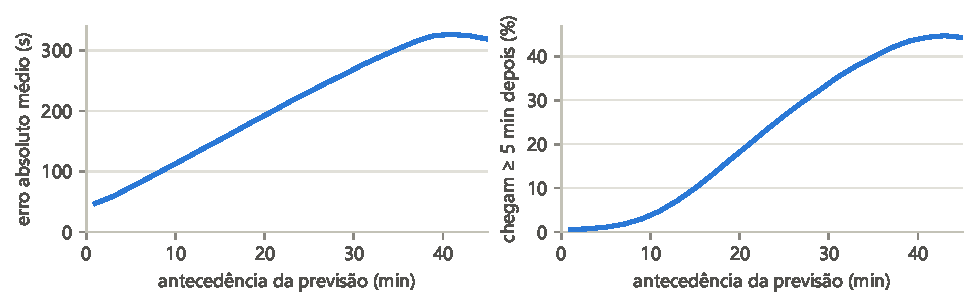
\includegraphics[width=\textwidth]{figuras/erro-previsao.pdf}
\caption{Erro absoluto médio (esquerda) e chegadas 5~min ou mais depois do
previsto (direita) por antecedência. Acima de 45~min, a janela de casamento de
60~min subestima o erro.}
\label{fig:previsao}
\end{figure}

\subsection{Limitações}

A referência ainda é a mediana da própria semana, e não a programação de ciclos,
o que torna a proporção de atrasados quase uniforme entre regiões. A chegada é
estimada por interpolação, com viés de alguns segundos nas paradas de embarque
intenso. A coleta pausou entre 1h e 4h, e uma única semana, com o feriado de
07/09 e linhas escolhidas pela disponibilidade de previsão, não cobre
sazonalidade nem é amostra aleatória da rede.
